\begin{frame}{Structure of the course}
    \begin{itemize}
        \item \alert{Moodle:} \url{https://go.epfl.ch/error-control}
        \vspace{-0.3em}
    \item \alert{ED Forum:} Announcements \& \alert{student-driven} discussion
        \vspace{1.0em}
        \item Lectures split into two rough segments
            \begin{itemize}
                \vspace{-0.3em}
                \item \alert{First half:} Matrix eigenvalue problems \& floating-point error
                \vspace{-0.3em}
                \item \alert{Second half:} Operator theory \& discretisation error
                \vspace{-0.3em}
                \item \alert{Notes:} \url{https://teaching.matmat.org/error-control}
            \end{itemize}
        \vspace{1.0em}
        \item Attendance of exercises is \alert{expected} \textcolor{grey5}{(introduces new material!)}
            \begin{itemize}
                \vspace{-0.3em}
                \item Discussion follows weekly exercise sheet
            \end{itemize}
    \end{itemize}
\end{frame}

\begin{frame}{Course evaluation}
    \begin{itemize}
        \item Marked semester project \textcolor{grey5}{($1/3$ of grade)}
        \item Project interview \& oral exam \textcolor{grey5}{($2/3$ of grade)}
        \item Project done in \alert{teams of $2-3$ students}.
        \item Interdisciplinary teams are highly recommended
        \vspace{1.5em}
        \item Working on the projects
            \alert{requires substantial time outside class}
            \begin{itemize}
                \vspace{-0.3em}
            \item[$\Rightarrow$] We will setup \alert{survey} in week 2 to \alert{aid formation of groups}
            \end{itemize}
    \end{itemize}
\end{frame}

\begin{frame}{Details on the exercises \& problem sheets}
    \begin{itemize}
        \item One problem sheet per week from moodle: \url{https://go.epfl.ch/error-control}
        \vspace{1em}
        \item Handing in of exercise sheets is optional
            \begin{itemize}
                \vspace{-0.3em}
                \item Submission can only be done in the project group
                \vspace{-0.3em}
                \item Tutors give feedback on submitted sheets
            \end{itemize}
        \vspace{1em}
        \item Initial exercises classes will be denser
        \item Later exercise classes provide time to work on the project
        \vspace{1em}
    \item \alert{Important:}
        \begin{itemize}
            \vspace{-0.3em}
            \item \textbf{Bring your laptop} to the exercise sessions
            \vspace{-0.3em}
            \item \textbf{Install \julia} programming language \textbf{beforehand}
            \vspace{-0.3em}
            \item[$\Rightarrow$] See \alert{instructions on moodle}
        \end{itemize}
    \end{itemize}
\end{frame}

\begin{frame}{Details on the project}
    \begin{itemize}
        \vspace{-0.3em}
        \item Project is essentially a larger problem sheet
        \vspace{-0.3em}
        \item One joint solution is submitted by each group
        \vspace{-0.3em}
        \item Responsibilities should be shared equally.
        \vspace{1.0em}
        \item During the oral exam \textcolor{grey5}{(about half the time)}
            \begin{itemize}
                \vspace{-0.3em}
                \item Presentation of the problem sheet by student
                \vspace{-0.3em}
                \item Targeted follow-up questions
                \vspace{-0.3em}
                \item \textcolor{grey5}{(The other half of the oral
                    is about general course understanding)}
            \end{itemize}
        \vspace{1.0em}
        \item Project evaluation criteria:
            \begin{itemize}
                \vspace{-0.3em}
                \item See document on moodle
            \end{itemize}
        \vspace{1.0em}
        \item Each group member obtains an \alert{individual mark}.
    \end{itemize}
\end{frame}

\begin{frame}{Topic of the semester project}
    \begin{itemize}
        \item Topic: \alert{Band structures with guaranteed error bars}
            \begin{itemize}
                \vspace{-0.5em}
                \item Handout: 21st October \textcolor{grey5}{(tentative)}
                \vspace{-0.5em}
                \item Duration: 2 months, i.e.~projected deadline: \textbf{20th December}
            \end{itemize}
        \vspace{1.5em}
        \begin{center}
        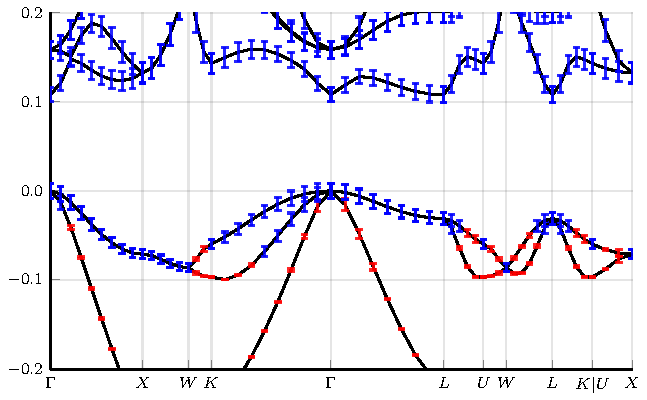
\includegraphics[width=0.7\textwidth]{img/si_band_errors.pdf}
        \end{center}
        \vspace{0.5em}
        \item Let's have a brief look at last year's projects \ldots
    \end{itemize}
\end{frame}

\begin{frame}{Group dynamics and mediation}
    \begin{itemize}
        \item Team work involves people
        \item People means tensions
            \begin{itemize}
                \vspace{-0.3em}
                \item \ldots and potentially unfair distribution of work
                \vspace{-0.3em}
                \item This is not unusual in academic and industry teams !
            \end{itemize}
        \vspace{1.0em}
        \item Additional \alert{learning goals of this course}:
            \begin{itemize}
                \item Learning to distribute work
                \item Learning to coordinate as a team
                \item Learning to resolve conflicts
            \end{itemize}
        \vspace{1.0em}
            \item \alert{You are not on your own}
                \begin{itemize}
                \vspace{-0.3em}
                \item We can provide support and mediate
                \end{itemize}
            \vspace{0.5em}
            \item \textbf{But} we cannot assist you if you don't reach out
                \linebreak
                \textbf{Hint:}  After the exam is too late
    \end{itemize}
\end{frame}

\begin{frame}{Questions ?}
    \begin{center}
        \huge{Questions ?}
    \end{center}
\end{frame}
